\subsection*{Architecture}
\underline{Exemple de shéma d'architecture:}
\begin{enumerate}[topsep=0pt, partopsep=0pt, itemsep=0pt, parsep=0pt]
    \item Quand les données sont prêtes, I2S IN génère une IRQ
    \item Le processeur répond à l'IRQ en activant le DMA pour transferer les données vers la mémoire.
    \item Le processeur active le block FFT qui lis les données de la mémoire externe et génère une IRQ une fois la FFT terminée.
    \item Le processeur effectue ses calculs à parir des données venant du block FFT.
    \item Le processeur active le block iFFT qui les données du processeur et génère une IRQ une fois la iFFT terminée.
    \item Le processeur répond à l'IRQ en activant le DMA pour transfert de données vers la mémoire.
    \item I2S OUT génère une IRQ quand il est prêt à lire les données avec le DMA. Il lis les données et les envoie sur le bus I2S ensuite il génère une interrupttion une fois qu'il a fini.
\end{enumerate}
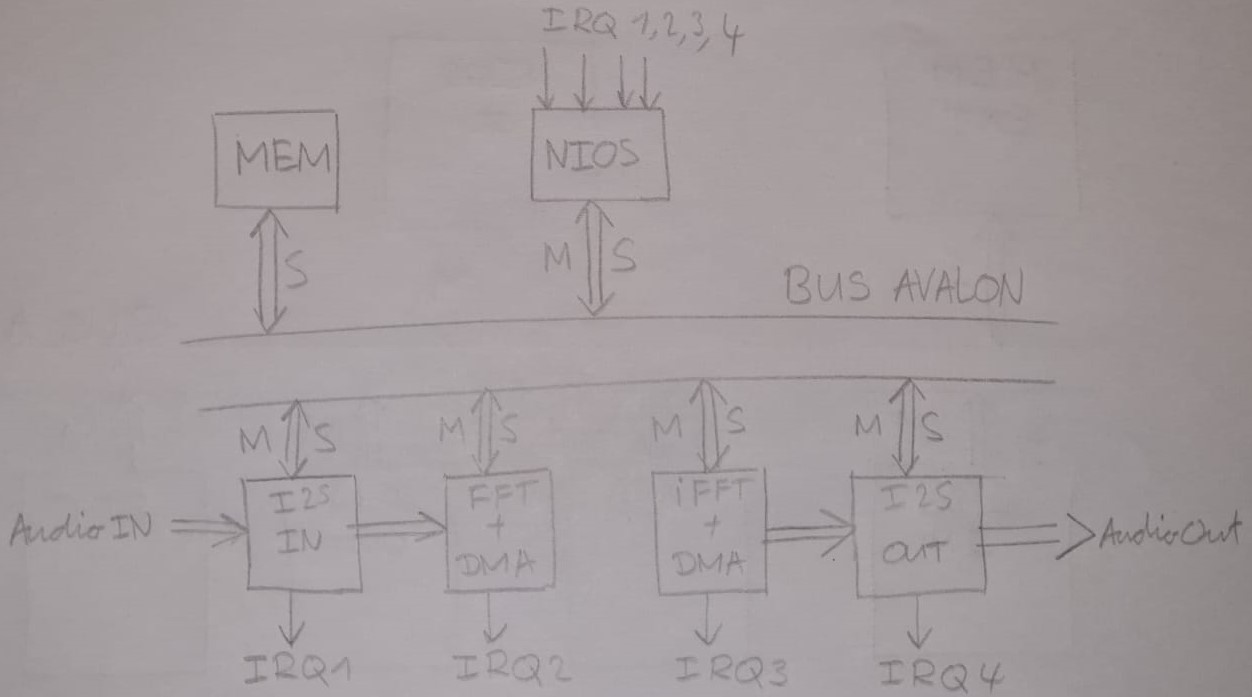
\includegraphics[width=\columnwidth]{images/schema_exa_ex1.jpg}
\underline{Exemple d'identity port:}
\begin{minted}{vhdl}
entity i2s_out is
    port (
        -- Avalon slave interface
        clock : in std_logic;
        reset : in std_logic;
        address : in std_logic_vector(1 downto 0);
        read : in std_logic;
        write : in std_logic;
        write_data : in std_logic_vector(31 downto 0);
        waitrequest : out std_logic;
        read_data : out std_logic_vector(31 downto 0);
        -- I2S interface for D/A
        sdim : out std_logic;
        lrclk : out std_logic;
        mclk : in std_logic;
        dem_sclk : in std_logic;
    );
end i2s_out;
\end{minted}

\underline{Exemple de modèle de registre:}

\begin{table}[H]
    \centering
    \begin{tabularx}{\columnwidth}{
            @{}
            >{\hsize=0.5\hsize}X % 1st column, 20% smaller
            >{\hsize=0.95\hsize}X % 2nd column, 20% smaller
            >{\hsize=0.95\hsize}X  % 3rd column, 20% smaller
            >{\hsize=0.4\hsize}X % 4th column, 20% smaller
            >{\hsize=2.05\hsize}X % 5th column, 80% larger
            @{}
        }
        \toprule
        Reg Address & Reg name C & Reg name VHDL & R/W & Description                                                                    \\
        \midrule
        1           & DATA       & dmaData       & W   & En soft pour passer les données brutes, en hard comme data input               \\
        2           & ADDR       & dmaAddr       & W   & Addresse à atteindre par le DMA                                                \\
        3           & SIZE       & dmaSize       & W   & Taille du mot à transmettre                                                    \\
        4           & STATUS     & dmaStatus     & W   & Dit si le DMA est libre                                                        \\
        5           & CONTROL    & control       & W   & 0 reset, 1 raw data, 2 channel when raw data or launch DMA, 3 anable interrupt \\
        6           & FREQ       & freq          & W   & Fréquence d'opération de la communication sérielle                             \\
        \bottomrule
    \end{tabularx}
\end{table}

\underline{Différence streaming et memory mapped:}\\
Le streaming permet de réduire la latence et la bandepassante nécessaire pour le transfert
car les datas peuvent être envoyées et reçues en continu. La méthode memory-mapped est plus
flexible et moins complexe à implémenter